\documentclass[conference]{IEEEtran}
\IEEEoverridecommandlockouts

\usepackage{cite}
\usepackage{amsmath,amssymb,amsfonts}
\usepackage{algorithm}
\usepackage{algorithmic}
\usepackage{graphicx}
\usepackage{textcomp}
\usepackage{xcolor}
\usepackage{booktabs}
\usepackage{array}
\usepackage{multirow}
\usepackage{tabularx}
\usepackage{caption}
\usepackage{subcaption}
\usepackage{url}
\usepackage{tikz}
\usetikzlibrary{shapes.geometric,arrows.meta,positioning,fit,calc}
\usepackage{hyperref}
\hypersetup{hidelinks}

\def\BibTeX{{\rm B\kern-.05em{\sc i\kern-.025em b}\kern-.08em
    T\kern-.1667em\lower.7ex\hbox{E}\kern-.125emX}}

\begin{document}

\title{A Multi-Pillar Prompt Quality Evaluation System Using Rule-Based, Semantic-Structural, Information-Theoretic, and Discourse Graph Metrics Without LLM Judgment}

\author{
\IEEEauthorblockN{Ojasvi Poonia}
\IEEEauthorblockA{Department of Computer Science and Engineering\\
M S Ramaiah Institute of Technology\\
Bengaluru, India\\
Email: 1ms23cs125@msrit.edu}
\and
\IEEEauthorblockN{Brunda G}
\IEEEauthorblockA{Department of Computer Science and Engineering\\
M S Ramaiah Institute of Technology\\
Bengaluru, India\\
Email: brundag@msrit.edu}
\thanks{Source code, the 20-prompt benchmark corpus with its measured scores, the benchmark and ablation scripts, and the test suite are available at \url{https://github.com/Ojasvi-Poonia/Prompt-Quality-Evaluator} under the MIT License.}
}

\maketitle

\begin{abstract}
Grading an LLM prompt today usually means paying a second LLM to grade it. That bothered us for two reasons. The cost climbs with every call, and the verdict drifts between runs even when the input does not change. So we tried scoring the prompt itself, directly, using classical NLP and no neural inference at all. Our pipeline computes 41 metrics. They sit in four groups: rule-based patterns, TF-IDF plus word-vector semantics, information theory, and a discourse graph we run PageRank over. Those 41 numbers fold into eight rubric dimensions and a single final score. To check whether any of this tracks human-like judgment, we benchmarked it against Gemini 2.5 Flash Lite over 20 prompts spanning five quality tiers, and we report every prompt individually rather than just the summary. Pearson landed at 0.932 ($p < 10^{-8}$); Spearman at 0.893. Five of the eight dimensions correlate strongly with Gemini ($r \geq 0.69$), two are middling, and Conciseness trails badly. The two systems pick the same verdict label $40\%$ of the time, and land within one band $80\%$ of the time. Beyond the headline numbers we walk through five prompts case by case, ablate each pillar, and document four places where the pipeline simply fails. It runs offline. It returns the exact same answer on every call. It costs nothing per evaluation, and instead of one opaque number it tells you which of the 41 metrics dragged the score down. Code, tests, the benchmark corpus with its measured scores, and pinned dependencies are all public under MIT.
\end{abstract}

\begin{IEEEkeywords}
prompt engineering, natural language processing, classical NLP, discourse graph analysis, text quality assessment, lexical diversity, readability metrics
\end{IEEEkeywords}

\section{Introduction}

Try this. Take any prompt. Run it through Gemini, ask Gemini to score it, and write the number down. Run it again. The number will be different. We sat with this for a while when we noticed it. ``Write a Python function that sorts a list of integers in ascending order'' got us 65 on the first call. 70 on the second. 62 on the third. No call was wrong on its own. No call was stable either.

Somewhere around 2024, prompt engineering stopped being a hobby and turned into paid work \cite{prompteng_survey}. People now sit and refine a single prompt across dozens of revisions before it ever ships. Put a paid LLM judge in that loop and two problems show up together. First, the money. Every call bills by tokens, and revisions are not free. Second, and this is the one that wasted our afternoon, the score moves between calls. You change one clause, the number goes up, and you genuinely cannot tell whether your edit helped or the judge just rolled a different value that minute. Picture a small team running 100 evaluation calls per prompt during development, across a thousand prompts in a year. The invoice is not pleasant.

The tools that already exist solve a nearby problem, not this one. Promptfoo \cite{promptfoo}, DeepEval \cite{deepeval}, and LangSmith \cite{langsmith} all run the prompt through a model and grade whatever comes back. The output gets judged. The prompt itself does not. So there is still no clean way to ask the obvious question, ``is this prompt worth sending,'' without first paying to send it.

We went the other way. Score the prompt text on its own, before any generation, with plain classical NLP. spaCy for parsing. TF-IDF, word frequency tables, n-gram entropy, parse-tree depth, a sentence-level discourse classifier, and a NetworkX graph that PageRank runs over. None of these are new ideas; that is rather the point. Nothing in the pipeline touches a neural network at evaluation time. Out the other end comes one score in $[0, 100]$, the eight dimension scores behind it, and 41 individual metric readings, each with a plain-English finding attached.

We claim four contributions:
\begin{enumerate}
\item A precise catalogue of 41 prompt-quality metrics, each with a mathematical or algorithmic definition, grouped into four pillars: rule-based, semantic-structural, information-theoretic, and discourse graph.
\item A discourse graph component that buckets every sentence as context, task, constraint, or example, builds a directed graph weighted by shared noun chunks and named entities, then runs PageRank over it to surface the focal sentence and information hierarchy.
\item A real benchmark against Gemini 2.5 Flash Lite on 20 prompts across five quality tiers, with overall and per-dimension Pearson and Spearman, plus five per-prompt case studies that take the disagreements apart.
\item Four ablation runs (one per pillar) and four failure modes, including the cases where the pipeline loses to the LLM and the cases where it wins.
\end{enumerate}

Is it actually deterministic? We ran one prompt a hundred times to find out. Same score every time, down to the last decimal. It runs with no network. It bills nothing. On a 2024 MacBook Pro the whole thing finishes in about two seconds, which made it 2--3 times quicker than the LLM judge in the runs we timed. The code and the tests are both public.

\section{Related Work}

\subsection{LLM-as-judge}
Most current work lives under the LLM-as-judge banner. G-Eval \cite{geval} hands GPT-4 a chain-of-thought rubric and reads the numbers back out. MT-Bench \cite{mtbench} does the same trick for multi-turn conversations. Prometheus \cite{prometheus} goes a step further and fine-tunes a smaller open model to be the judge, which shaves the inference bill without removing it. The shared weakness runs through all three. The judge is a black box. The cost keeps adding up. And the result will not reproduce, because even at temperature zero, caching, batching, and silent version bumps mean two identical calls can disagree.

The same pattern shows up wrapped in tooling: Promptfoo \cite{promptfoo}, DeepEval \cite{deepeval}, LangSmith \cite{langsmith}, Braintrust \cite{braintrust}, RAGAS \cite{ragas}. All of them grade what the model produces, never the prompt that produced it. A generation call has to happen first, and you pay for it.

\subsection{Classical text quality assessment}
Scoring text without a transformer is not new; automated essay scoring goes back to the 1960s. ETS built e-rater \cite{erater} out of dozens of hand-engineered features (syntactic complexity, vocabulary, discourse structure, mechanics) fed into shallow classifiers. Coh-Metrix \cite{cohmetrix} pushes that to well over a hundred features aimed at cohesion and coherence. Both have been checked against human raters for decades, and both still ship commercially. We leaned on this lineage heavily.

Readability carries its own history. Flesch-Kincaid \cite{flesch} came out of a 1975 US Navy report. Coleman-Liau \cite{coleman} trades syllable counts for character counts. ARI, Gunning Fog, SMOG \cite{smog}, and Linsear Write each grab a slightly different facet of difficulty. The lesson education researchers learned long ago is that no one formula suffices, so they average a handful. We do too.

\subsection{Lexical diversity}
Type-Token Ratio (TTR) is the old measure, and it has a known length-bias problem that makes cross-document comparison shaky \cite{mccarthy_jarvis_2010}. McCarthy and Jarvis introduced MTLD specifically to fix this \cite{mtld}. HD-D uses a hypergeometric distribution to give an expected diversity that does not depend on text length. MATTR averages TTR over a sliding window.

\subsection{Discourse analysis}
Rhetorical Structure Theory \cite{rst} draws a document as a tree of nucleus and satellite units, joined by relations like elaboration, contrast, condition, or example. The Penn Discourse Treebank \cite{pdtb} takes a different angle, keying off the discourse connectives themselves. Graphs built from discourse structure have shown up in essay scoring \cite{guinaudeau_strube} and summarisation evaluation \cite{xu_disco}. What we could not find was anyone pointing the technique at LLM prompt quality, which is where Pillar 4 comes in.

\subsection{Position of this work}
So we sit at an intersection. Pillars 1 and 3 borrow classical text-quality features. Pillar 2 is TF-IDF and word vectors. Pillar 4 is a discourse graph we built from scratch. What is new here is the metric catalogue tuned specifically for prompts, the discourse-graph pillar, and the head-to-head against an LLM judge.

\section{Problem Formulation}

Here is the task stated cleanly. Let $T$ be the set of possible prompt texts, and let $D = \{d_1, \ldots, d_8\}$ name the eight rubric dimensions we score against: Clarity, Specificity, Structure, Task Definition, Context Completeness, Constraint Specification, Information Richness, and Conciseness.

A prompt scorer is a function:
\[ S : T \to [0, 1]^8 \times [0, 100] \times \mathcal{F} \]
The first slot is the per-dimension scores, the second is the aggregated final score, and $\mathcal{F}$ holds the textual findings (one or more per metric).

Four constraints sit on $S$, and we treated them as hard requirements rather than nice-to-haves:
\begin{itemize}
\item \textbf{Deterministic}: $S(t)$ has to return the same value every call, for any $t$.
\item \textbf{Offline}: no network round-trips during evaluation.
\item \textbf{Transformer-free}: no neural inference at scoring time. Pre-trained word vector tables and static rule tables are fine. Transformer models are not.
\item \textbf{Explainable}: every component of the output has to be traceable back to one or more named features.
\end{itemize}

LLM-as-judge fails the first three outright. A single-formula heuristic like raw word count or bare Flesch-Kincaid passes the first three but fails the fourth, because one number cannot tell a user the specific thing to fix.

\section{System Architecture}

The layout is simple enough to hold in your head. Four pillars run in parallel. A rubric mapper sits below them, then three multiplicative modifiers, then a formatter that emits the final score and the per-metric findings. Figure \ref{fig:arch} traces the dataflow end to end.

\begin{figure}[t]
\centering
\resizebox{\columnwidth}{!}{%
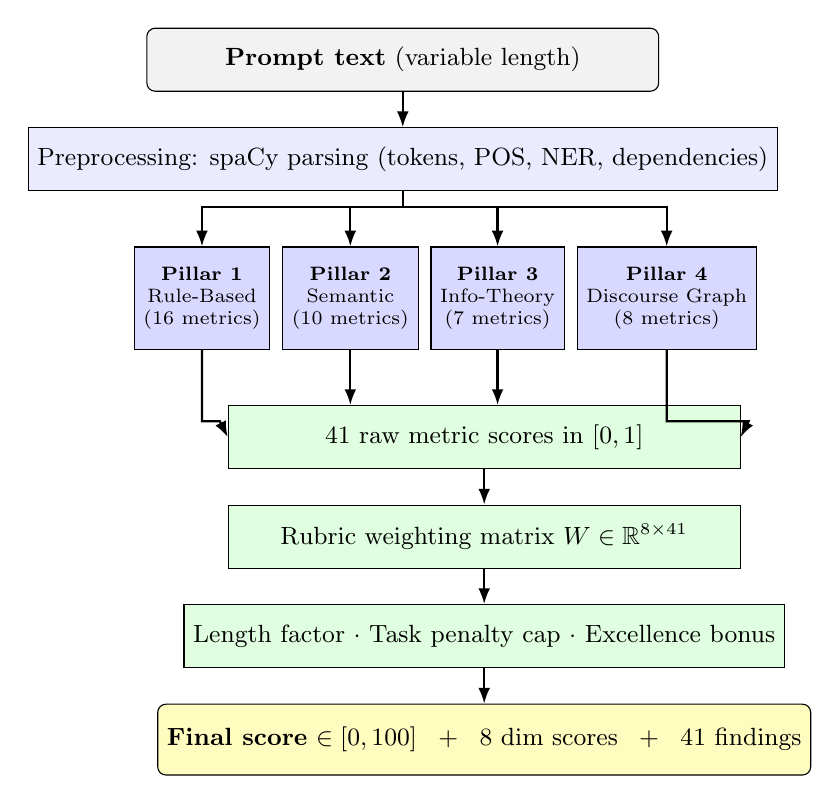
\begin{tikzpicture}[
  node distance=0.45cm,
  every node/.style={font=\small},
  io/.style={rectangle, draw, rounded corners=3pt, fill=gray!10, minimum width=6.5cm, minimum height=0.8cm, align=center},
  proc/.style={rectangle, draw, fill=blue!8, minimum width=6.5cm, minimum height=0.8cm, align=center},
  pillar/.style={rectangle, draw, fill=blue!15, minimum width=1.55cm, minimum height=1.3cm, align=center, font=\scriptsize},
  agg/.style={rectangle, draw, fill=green!12, minimum width=6.5cm, minimum height=0.8cm, align=center},
  outbox/.style={rectangle, draw, rounded corners=3pt, fill=yellow!25, minimum width=6.5cm, minimum height=0.9cm, align=center},
  arrow/.style={-{Latex[length=2mm]}, thick}
]
\node[io] (in) {\textbf{Prompt text} (variable length)};
\node[proc, below=of in] (parse) {Preprocessing: spaCy parsing (tokens, POS, NER, dependencies)};

\node[pillar, below=0.7cm of parse, xshift=-2.55cm] (p1) {\textbf{Pillar 1}\\Rule-Based\\(16 metrics)};
\node[pillar, right=0.15cm of p1] (p2) {\textbf{Pillar 2}\\Semantic\\(10 metrics)};
\node[pillar, right=0.15cm of p2] (p3) {\textbf{Pillar 3}\\Info-Theory\\(7 metrics)};
\node[pillar, right=0.15cm of p3] (p4) {\textbf{Pillar 4}\\Discourse Graph\\(8 metrics)};

\node[agg, below=0.7cm of p2.south, xshift=1.7cm] (raw) {41 raw metric scores in $[0, 1]$};
\node[agg, below=of raw] (rub) {Rubric weighting matrix $W \in \mathbb{R}^{8 \times 41}$};
\node[agg, below=of rub] (mod) {Length factor $\cdot$ Task penalty cap $\cdot$ Excellence bonus};
\node[outbox, below=of mod] (out) {\textbf{Final score} $\in [0, 100]$ \, + \, 8 dim scores \, + \, 41 findings};

\draw[arrow] (in) -- (parse);
\draw[arrow] (parse.south) -- ++(0,-0.2) -| (p1.north);
\draw[arrow] (parse.south) -- ++(0,-0.2) -| (p2.north);
\draw[arrow] (parse.south) -- ++(0,-0.2) -| (p3.north);
\draw[arrow] (parse.south) -- ++(0,-0.2) -| (p4.north);
\draw[arrow] (p1.south) |- ($(raw.west) + (-0.1,0.2)$) -- (raw.west);
\draw[arrow] (p2.south) -- (raw.north -| p2.south);
\draw[arrow] (p3.south) -- (raw.north -| p3.south);
\draw[arrow] (p4.south) |- ($(raw.east) + (0.1,0.2)$) -- (raw.east);
\draw[arrow] (raw) -- (rub);
\draw[arrow] (rub) -- (mod);
\draw[arrow] (mod) -- (out);
\end{tikzpicture}%
}
\caption{System architecture. One text input goes through preprocessing, then the four pillars in parallel. Their 41 outputs feed a fixed weighting matrix that yields eight dimension scores. Three multiplicative adjustments produce the final number.}
\label{fig:arch}
\end{figure}

Disk footprint at evaluation time is about 700 MB. Almost all of it is two files: the spaCy \texttt{en\_core\_web\_md} model at 40 MB, and the Java grammar tables that come bundled with language-tool-python, which alone are around 600 MB. Memory peaks near 1.5 GB while a prompt is scored. There is no GPU anywhere in the loop, and no network call.

\section{The 41 Metrics}

Below is the full catalogue. For each metric we give the inputs, the formula or the algorithm, and the range. Every one returns a value in $[0, 1]$ together with at least one textual finding that ends up in the report.

\subsection{Pillar 1: Rule-Based Metrics}

\textbf{M1. length} ($\ell$). Word count $w$ of the prompt. Score is a Gaussian centred at 150 words:
\[ \ell(t) = \exp\!\left(-\tfrac{1}{2}\left(\tfrac{w - 150}{200}\right)^2\right) \]
with hard penalties: if $w < 10$, multiply by $0.3$; if $w > 2000$, multiply by $0.5$.

\textbf{M2. grammar}. LanguageTool \cite{languagetool} matches $g$ plus pyspellchecker typo count $\tau$, normalised by sentence count $s$:
\[ \mathrm{grammar}(t) = \max\!\left(0,\ 1 - 0.3 \cdot \tfrac{g + \tau}{s}\right) \]
Code blocks are stripped before checking; we found fenced code triggers false grammar errors at a high rate.

\textbf{M3. readability}. Six readability formulas are averaged: Flesch-Kincaid \cite{flesch}, Coleman-Liau \cite{coleman}, ARI, Gunning Fog, SMOG \cite{smog}, and Linsear Write. The mean grade $\bar{g}$ is mapped through a Gaussian centred at grade 10:
\[ \mathrm{readability}(t) = \exp\!\left(-\tfrac{1}{2}\left(\tfrac{\bar{g} - 10}{4}\right)^2\right) \]

\textbf{M4. specificity}. Density of concrete details per sentence. Count $n_e$ named entities, $n_n$ numeric values, $n_t$ technical terms (words with zipf score $<$ 4.5), $n_q$ quoted strings, and $n_c$ code-like tokens. Typo-flagged words are excluded. If typo count is $k$:
\[ \mathrm{specificity}(t) = \max\!\left(0,\ \tfrac{n_e + n_n + n_t + n_q + n_c}{8 s} - 0.2 k\right) \]

\textbf{M5. structure}. Detection score from regex patterns (bullets, numbered lists, markdown headers, fenced code, horizontal rules, section labels) combined with a markdown-it-py bonus for well-formed lists, headers with content, and nested structures. The final structure score blends variety (number of distinct element types) and count (total elements).

\textbf{M6. task\_signal}. Detection score from three signal classes: imperative verbs in a 30-verb lexicon (\texttt{write}, \texttt{explain}, \texttt{generate}, \ldots), question patterns (\texttt{what}, \texttt{how}, \texttt{why}, $\ldots$ followed by \texttt{?}), and deliverable nouns (\texttt{code}, \texttt{json}, \texttt{table}, \ldots). Each class contributes up to a maximum cap.

\textbf{M7. constraint}. Constraint signals across five categories: negations (\texttt{do not}, \texttt{avoid}, \texttt{never}), limits (\texttt{maximum}, \texttt{at most}), format directives (\texttt{in json}, \texttt{as a table}), audience specs (\texttt{for beginners}, \texttt{for experts}), and tone directives (\texttt{formal}, \texttt{concise}, \texttt{technical}). Score combines category variety and total count.

\textbf{M8. contradiction}. Detection of logical conflicts: incompatible word/sentence counts, opposing tone pairs (\texttt{formal} with \texttt{casual}), mutually exclusive instructions (\texttt{include examples} with \texttt{do not include examples}). Returns $0.5$ (neutral) when no constraint signals are present, which avoids vacuous-truth inflation on bare prompts.

\textbf{M9. reference\_similarity}. Maximum cosine similarity between the user prompt and any canonical prompt in the detected domain. We maintain 1--2 hand-curated canonical prompts per domain (coding, creative, analysis, instructional, general). Using spaCy \texttt{en\_core\_web\_md} document vectors:
\[ \mathrm{ref\_sim}(t) = \max_{p \in \mathcal{C}_{\text{dom}(t)}} \tfrac{\mathbf{v}(t) \cdot \mathbf{v}(p)}{\|\mathbf{v}(t)\| \, \|\mathbf{v}(p)\|} \]
where $\mathcal{C}_d$ is the canonical set for domain $d$ and $\mathbf{v}(\cdot)$ is the document vector.

\textbf{M10. persona\_signal}. Pattern detection for role-setting phrases (\texttt{you are a senior X}, \texttt{act as Y}, \texttt{imagine you are Z}) plus NER-derived role specificity. A prompt that names a domain expert role scores higher than one with a generic role.

\textbf{M11. few\_shot\_quality}. Detection of in-context examples: Input/Output pairs, numbered \texttt{Example:} labels, and arrow mappings (\texttt{foo -> bar}). Score scales from $0.55$ (one example) up to $0.95$ (three or more examples in canonical form).

\textbf{M12. hedging}. Density of hedge phrases in a curated lexicon (\texttt{kind of}, \texttt{maybe}, \texttt{I think}, \texttt{perhaps}, \ldots, 33 items). High hedging density signals uncertainty, which thins out instruction clarity.

\textbf{M13. safety}. Detection of prompt-injection patterns (\texttt{ignore previous instructions}, \texttt{disregard all rules}, \texttt{system:}, \ldots). Score starts at $1.0$ and drops $0.3$ per detected pattern. This is a guardrail, not a quality metric in the usual sense.

\textbf{M14. output\_schema}. Detection of explicit output format specifications: JSON blocks in code fences, TypeScript type definitions, YAML schemas with type annotations, function/class signatures, and typed field lists. Score scales by the number and quality of schema-like structures.

\textbf{M15. compound\_task\_count}. Counts distinct task verbs chained via spaCy dependency conjunctions. A prompt that says ``read the CSV, filter rows, compute the mean, sort by department, and export'' has five chained tasks. Score rewards 2--6 chained tasks and penalises 8+ as over-stuffed.

\textbf{M16. imperative\_strength}. POS-tagged sentence-initial verbs minus politeness softeners. ``Write a function'' is a strong imperative. ``Could you please maybe write a function'' is the same intent with three softeners attached. Score:
\[ \mathrm{imp\_str}(t) = 0.7 + 0.1 \cdot [\text{imp} \geq 2] + 0.1 \cdot [\text{soft} = 0] + 0.05 \cdot [\text{caps}] \]
where the brackets are indicators.

\subsection{Pillar 2: Semantic-Structural Metrics}

\textbf{M17. coherence}. Cosine similarity between consecutive sentences. We compute it two ways and blend: lexical (TF-IDF, weight 0.4) and semantic (spaCy md word vectors, weight 0.6). For sentences $s_i, s_{i+1}$:
\[ \mathrm{coh}_i = 0.4 \cdot \cos\bigl(\mathbf{v}^{\text{tf}}(s_i), \mathbf{v}^{\text{tf}}(s_{i+1})\bigr) + 0.6 \cdot \cos\bigl(\mathbf{v}^{\text{w}}(s_i), \mathbf{v}^{\text{w}}(s_{i+1})\bigr) \]
The metric returns the mean across all consecutive pairs, scaled by $1.3$.

\textbf{M18. semantic\_density}. Ratio of unique meaningful lemmas to total tokens:
\[ \mathrm{sem\_dens}(t) = \min\!\left(1,\ 2.5 \cdot \tfrac{|\{\mathrm{lemma}(w) : \mathrm{pos}(w) \in \{\text{N}, \text{V}, \text{Adj}, \text{Adv}\}\}|}{|\text{tokens}|}\right) \]
Lemmas are deduplicated and stop-words excluded.

\textbf{M19. topic\_focus}. Mean cosine distance of each sentence to the document centroid, using both TF-IDF and vector representations:
\[ d_{\text{tf}} = \tfrac{1}{n}\sum_i (1 - \cos(\mathbf{v}^{\text{tf}}(s_i), \bar{\mathbf{v}}^{\text{tf}})) \]
\[ d_{\text{w}} = \tfrac{1}{n}\sum_i (1 - \cos(\mathbf{v}^{\text{w}}(s_i), \bar{\mathbf{v}}^{\text{w}})) \]
\[ \mathrm{focus}(t) = \max\!\left(0,\ 1 - 1.6 (0.4 d_{\text{tf}} + 0.6 d_{\text{w}})\right) \]

\textbf{M20. lexical\_sophistication}. Word rarity score using zipf frequencies from \texttt{wordfreq} \cite{wordfreq}. For each content word $w$ with zipf score $z(w) \in [0, 8]$:
\[ r(w) = \begin{cases}
0.10 & z(w) \geq 6.5 \\
0.30 & 5.0 \leq z(w) < 6.5 \\
0.55 & 3.5 \leq z(w) < 5.0 \\
0.75 & 2.0 \leq z(w) < 3.5 \\
0.85 & 1.0 \leq z(w) < 2.0 \\
0.80 & z(w) < 1.0 \text{ but in tech vocab or spaCy has vector} \\
0.0  & \text{otherwise (likely typo)}
\end{cases} \]
The metric returns $\min(1, 0.3 + 0.7 \bar{r})$ where $\bar{r}$ is the mean over content words.

\textbf{M21. sentence\_flow}. Coefficient of variation of sentence lengths. Let $\sigma$ and $\mu$ be the standard deviation and mean of sentence word counts. The metric is a Gaussian centred at $\mathrm{CV} = 0.45$ with $\sigma = 0.3$:
\[ \mathrm{flow}(t) = \exp\!\left(-\tfrac{1}{2}\left(\tfrac{\sigma/\mu - 0.45}{0.3}\right)^2\right) \]
Robotic uniformity ($\mathrm{CV} \approx 0$) and chaotic variance ($\mathrm{CV} > 0.8$) both lose points.

\textbf{M22. reference\_resolution}. Counts ambiguous pronouns (\texttt{it}, \texttt{this}, \texttt{that}, \texttt{they}, \ldots) in subject or object position via spaCy dependency parse, then checks whether a noun antecedent exists in the current or previous sentence. The metric returns:
\[ \mathrm{ref\_res}(t) = 1 - \tfrac{\text{ambiguous}}{\text{total pronouns}} \]
A neutral $0.5$ comes back when the prompt is too short to evaluate.

\textbf{M23. tone\_consistency}. Variance of VADER compound sentiment scores \cite{vader} across sentences. Cross-tone prompts (strong positive and strong negative sentences mixed) get penalised:
\[ \mathrm{tone}(t) = \max(0, 1 - 3 \sigma^2_{\text{VADER}}) \]

\textbf{M24. objectivity}. Inverse of TextBlob subjectivity score $s_{\text{tb}} \in [0, 1]$:
\[ \mathrm{obj}(t) = 1 - 0.7 s_{\text{tb}} \]
Subjective phrasings (``I think'', ``I feel'', ``it would be nice'') lower the score.

\textbf{M25. syntactic\_complexity}. Mean dependency-tree depth $\bar{d}$ and mean clause count per sentence $\bar{c}$, blended through two Gaussians:
\[ \mathrm{syn}(t) = 0.6 \exp\!\left(-\tfrac{1}{2}\left(\tfrac{\bar{d} - 5.5}{2.5}\right)^2\right) + 0.4 \exp\!\left(-\tfrac{1}{2}\left(\tfrac{\bar{c} - 2}{1.5}\right)^2\right) \]

\textbf{M26. discourse\_markers}. Density of logical connectives across six categories: addition, contrast, cause, sequence, example, conclusion. We use a lexicon of 50+ markers drawn from PDTB \cite{pdtb}. Score scales with both density and category variety.

\subsection{Pillar 3: Information-Theoretic Metrics}

These metrics tokenise the prompt with tiktoken \texttt{cl100k\_base} (the same tokeniser GPT models use), then operate on the token sequence. Every Pillar 3 metric applies a short-text cap of $0.3$ for prompts under 30 tokens, because entropy-based measures are mathematically biased toward high scores on short text.

\textbf{M27. shannon\_entropy}. Normalised Shannon entropy over the token frequency distribution:
\[ H(t) = -\sum_i p_i \log_2 p_i,\quad p_i = \tfrac{f_i}{N} \]
\[ \mathrm{ent}(t) = \tfrac{H(t)}{\log_2 V} \]
where $N$ is total tokens, $f_i$ is the count of token type $i$, and $V$ is the number of distinct token types.

\textbf{M28. redundancy}. Inverse of token-level redundancy:
\[ R(t) = 1 - \tfrac{V}{N} \]
\[ \mathrm{red}(t) = \begin{cases} 1 - R(t) & R(t) \leq 0.6 \\ 0.5 (1 - R(t)) & R(t) > 0.6 \end{cases} \]
The piecewise function applies a heavy penalty when more than $60\%$ of tokens are repeats.

\textbf{M29. information\_density}. Entropy per token:
\[ \mathrm{ID}(t) = \min(1,\ 10 \cdot H(t) / N) \]

\textbf{M30. vocabulary\_richness}. Mean of four lexical diversity measures: basic TTR, MTLD with threshold $0.72$, HD-D with $42$ draws, and MATTR with window 10:
\[ \mathrm{voc}(t) = \tfrac{1}{4}(\mathrm{TTR} + \widehat{\mathrm{MTLD}} + \widehat{\mathrm{HD\text{-}D}} + \widehat{\mathrm{MATTR}}) \]
where each component is normalised to $[0, 1]$. The MTLD/HD-D/MATTR triple is implemented via \texttt{lexicalrichness} and is known to be length-robust \cite{mtld}.

\textbf{M31. ngram\_repetition}. Counts repeated bigrams and trigrams. For $n$-grams $g_n$:
\[ r_n = \tfrac{|\{g : \mathrm{count}(g) > 1\}|}{|\{g\}|} \]
\[ \mathrm{ngram}(t) = \max(0,\ 1 - 3 \cdot \tfrac{r_2 + r_3}{2}) \]
The $3 \times$ amplification penalises moderate repetition heavily.

\textbf{M32. burstiness}. Variance of Shannon entropy across five equal token-chunks of the prompt. Low variance points to consistent information flow; high variance to alternating dense regions and filler:
\[ \mathrm{burst}(t) = \max(0, 1 - 2 \sigma^2_{H_{\text{chunk}}}) \]

\textbf{M33. sentence\_repetition}. For each pair of sentences $s_i, s_j$, compute word overlap (Jaccard over content words). Count pairs with overlap $> 0.7$. Returns:
\[ \mathrm{sent\_rep}(t) = \max(0,\ 1 - 2 \cdot \tfrac{|\text{overlapping pairs}|}{|\text{total pairs}|}) \]

\subsection{Pillar 4: Discourse Graph Metrics}

Pillar 4 is the one we built from scratch, and it is the piece we think is most novel. Each sentence gets a discourse label, edges link sentences that share content, and standard graph algorithms turn the result into numbers.

\subsubsection{Sentence classification}
Take a sentence $s$, lowercase it, and run four regex pattern sets against it in a fixed priority order: EXAMPLE, then CONSTRAINT, then TASK, then CONTEXT. The patterns:
\begin{itemize}
\item EXAMPLE: \texttt{for example}, \texttt{e.g.}, \texttt{such as}, \texttt{for instance}, \ldots
\item CONSTRAINT: \texttt{must}, \texttt{should}, \texttt{do not}, \texttt{maximum}, \texttt{in json}, \texttt{format}, \ldots
\item TASK: \texttt{write}, \texttt{explain}, \texttt{analyse}, \ldots and question patterns
\item CONTEXT: \texttt{currently}, \texttt{given}, \texttt{i have}, \texttt{we are}, \texttt{the current}, \ldots
\end{itemize}
A sentence that matches none of them is labelled OTHER.

The priority order earns its place. Consider ``For example, write a function''. That sentence trips both an EXAMPLE marker and a TASK marker at once. We resolve the tie toward EXAMPLE, because in practice illustrative content almost never doubles as the prompt's real task once you read the whole thing.

\subsubsection{Graph construction}
We build a directed graph $G = (V, E)$, with $V$ the classified sentences. Edges go in over two passes:
\begin{enumerate}
\item Every consecutive pair $(s_i, s_{i+1})$ gets an edge $s_i \to s_{i+1}$ with weight 1. This keeps the reading order in the graph.
\item For any non-adjacent pair $(s_i, s_j)$, $j > i+1$, we intersect their noun chunks and named entities. A non-empty intersection adds an edge $s_i \to s_j$ weighted by how many items they share.
\end{enumerate}

The pseudocode is in Algorithm \ref{alg:graph}.

\begin{algorithm}[t]
\caption{Discourse Graph Construction}
\label{alg:graph}
\begin{algorithmic}[1]
\STATE \textbf{Input:} prompt text $t$
\STATE \textbf{Output:} directed graph $G = (V, E)$
\STATE $S \leftarrow$ split\_sentences($t$)
\STATE $V \leftarrow \emptyset$, $E \leftarrow \emptyset$
\FOR{$i = 0$ to $|S| - 1$}
    \STATE $\text{type}_i \leftarrow$ classify\_sentence($S_i$)
    \STATE $C_i \leftarrow$ noun\_chunks($S_i$)
    \STATE $N_i \leftarrow$ named\_entities($S_i$)
    \STATE $V \leftarrow V \cup \{(i, \text{type}_i, C_i, N_i)\}$
\ENDFOR
\FOR{$i = 0$ to $|S| - 2$}
    \STATE $E \leftarrow E \cup \{(i, i+1, 1)\}$
\ENDFOR
\FOR{$i = 0$ to $|S| - 3$}
    \FOR{$j = i+2$ to $|S| - 1$}
        \STATE $w \leftarrow |C_i \cap C_j| + |N_i \cap N_j|$
        \IF{$w > 0$}
            \STATE $E \leftarrow E \cup \{(i, j, w)\}$
        \ENDIF
    \ENDFOR
\ENDFOR
\RETURN $G = (V, E)$
\end{algorithmic}
\end{algorithm}

\subsubsection{Graph metrics}
\textbf{M34. completeness}. $0.33$ for each of CONTEXT, TASK, CONSTRAINT present in $V$; bonus $0.1$ for EXAMPLE.

\textbf{M35--M37. has\_context, has\_task, has\_constraint}. Binary indicators: $1.0$ if the corresponding type shows up in $V$, otherwise $0.0$.

\textbf{M38. connectivity}. Graph density divided by the number of weakly connected components:
\[ \mathrm{conn}(G) = \min(1,\ \tfrac{2 \cdot \rho(G)}{k}) \]
where $\rho(G) = |E| / (|V|(|V|-1))$ is the density and $k$ is the number of components.

\textbf{M39. information\_flow}. Average position of CONTEXT, TASK, and CONSTRAINT nodes. Score 1.0 if mean(CONTEXT) $<$ mean(TASK) $<$ mean(CONSTRAINT), otherwise lower. Two pairwise checks contribute $0.5$ each.

\textbf{M40. complexity}. Edge-to-node ratio, Gaussian-scored:
\[ \mathrm{cmplx}(G) = \exp\!\left(-\tfrac{1}{2}\left(\tfrac{|E|/|V| - 2.25}{1.5}\right)^2\right) \]

\textbf{M41. centrality}. Run PageRank \cite{pagerank} on $G$ with damping factor $\alpha = 0.85$. Compute coefficient of variation of the resulting PageRank scores:
\[ \mathrm{cent}(G) = \exp\!\left(-\tfrac{1}{2}\left(\tfrac{\sigma_{\text{PR}}/\mu_{\text{PR}} - 0.4}{0.3}\right)^2\right) \]
Read the two extremes this way. A flat PageRank distribution (CV $\approx 0$) means no sentence stands out as the focus. A spiked one (CV $> 0.8$) means a single sentence dominates while the rest add little. Neither is what a well-built prompt looks like, so both are penalised.

\section{Rubric Aggregation}

The 41 raw metrics collapse into eight dimensions through a fixed weighting matrix $W \in \mathbb{R}^{8 \times 41}$. Every row sums to one. Table \ref{tab:rubric} lists the weights in full.

\begin{table*}[t]
\centering
\caption{Rubric weighting matrix. Each row defines a dimension; weights sum to 1.0 within each row.}
\label{tab:rubric}
\small
\begin{tabularx}{\textwidth}{l X}
\toprule
\textbf{Dimension} & \textbf{Metric (weight)} \\
\midrule
Clarity & grammar (0.18), readability (0.15), reference\_resolution (0.10), sentence\_flow (0.10), tone\_consistency (0.08), objectivity (0.10), hedging (0.14), syntactic\_complexity (0.15) \\
\midrule
Specificity & specificity (0.30), reference\_similarity (0.10), output\_schema (0.15), lexical\_sophistication (0.20), semantic\_density (0.15), persona\_signal (0.10) \\
\midrule
Structure & structure (0.20), completeness (0.10), information\_flow (0.10), centrality (0.10), coherence (0.10), discourse\_markers (0.10), reference\_similarity (0.10), few\_shot\_quality (0.10), output\_schema (0.10) \\
\midrule
Task Definition & task\_signal (0.30), imperative\_strength (0.15), compound\_task\_count (0.10), has\_task (0.15), contradiction (0.10), persona\_signal (0.05), safety (0.15) \\
\midrule
Context Completeness & has\_context (0.30), topic\_focus (0.20), length (0.20), persona\_signal (0.15), few\_shot\_quality (0.15) \\
\midrule
Constraint Specification & constraint (0.35), has\_constraint (0.20), contradiction (0.15), output\_schema (0.20), safety (0.10) \\
\midrule
Information Richness & shannon\_entropy (0.25), vocabulary\_richness (0.25), information\_density (0.25), semantic\_density (0.25) \\
\midrule
Conciseness & redundancy (0.25), ngram\_repetition (0.25), sentence\_repetition (0.25), burstiness (0.25) \\
\bottomrule
\end{tabularx}
\end{table*}

Once the dimension scores $\mathbf{d} = W \mathbf{m}$ are in hand (with $\mathbf{m}$ the 41-dim vector of raw scores), three modifiers run on top.

\subsection{Modifier 1: length factor}
Short prompts get scaled down, because a four-word prompt simply has no room to demonstrate structure or context. With $w$ the word count:
\[ \lambda(w) = \begin{cases}
1.0 & w \geq 30 \\
0.4 & w \leq 3 \\
0.6 + 0.04(w - 3) & 3 < w \leq 10 \\
0.85 + 0.0075(w - 10) & 10 < w < 30
\end{cases} \]

\subsection{Modifier 2: task penalty cap}
When $\mathrm{task\_signal}(t) < 0.2$ and $\mathrm{has\_task}(t) < 0.5$, we clip the final score at:
\[ C(w) = \begin{cases}
12 & w \leq 5 \\
22 & 5 < w \leq 10 \\
32 & 10 < w \leq 20 \\
40 & w > 20
\end{cases} \]
The point is blunt: if there is no clear instruction, no amount of clean formatting should lift the prompt over this ceiling.

\subsection{Modifier 3: excellence bonus}
Write $p_1, p_2, p_3, p_4$ for the four pillar means. When even the weakest of the four clears $0.6$, we add a bonus:
\[ B = 0.25 (\overline{p} - 0.6) \]
with $\overline{p}$ the mean of the four. A prompt only collects this bonus by being good across the board, which is exactly the behaviour we want to encourage and the gaming we want to prevent.

\subsection{Final aggregation}
Let $\bar{d}$ be the mean dimension score after domain weighting. The final number is
\[ F(t) = \min\!\left(100,\ \min(C(w),\ 100 \cdot (\lambda(w) \bar{d} + B))\right) \]
Two minimums, two jobs. The inner one applies the task penalty cap. The outer one keeps the score from running past 100.

\section{Experimental Methodology}

\subsection{Benchmark corpus}
Our benchmark is 20 prompts, four to a tier, across five quality tiers:
\begin{itemize}
\item \textbf{Terrible}: 1--4 words, no task signal. ``help'', ``do thing'', ``write code'', ``fix it''.
\item \textbf{Poor}: vague, hedged, under 50 words. ``Write me a python script that does stuff with data''.
\item \textbf{Average}: functional but minimal, 30--80 words. ``Write a Python function that takes a list of numbers and returns the top 3 largest values. Handle edge cases like empty lists and lists with fewer than 3 elements.''
\item \textbf{Good}: structured with sections, 100--200 words. Multi-section coding and technical prompts.
\item \textbf{Excellent}: full Persona / Context / Task / Requirements / Constraints / Examples structure, 200--500 words.
\end{itemize}

The corpus carries tier labels only; it assigns no domain by hand. Run the domain detector over it and 11 of the 20 prompts come back as coding and the remaining 9 as general. The coding tilt is deliberate. That is where the bulk of real prompt-engineering effort goes, so it is where the scorer needs to be sharpest. It is also the clearest limitation of the benchmark, and Section \ref{sec:limitations} returns to it.

\subsection{LLM baseline}
Our judge is Gemini 2.5 Flash Lite. The judge prompt is structured: it names the eight dimensions, requests a $[0, 1]$ score for each, then asks for a short rationale and a $0$--$100$ final score. We set temperature to zero, though as noted earlier even that does not fully stop the drift between calls.

Every number we report about the judge depends on how the judge was elicited, so the judge itself ships with the repository rather than sitting behind a description. The exact prompt template, the temperature setting, and the response parsing are all in \texttt{llm\_evaluator/}. A reader who disagrees with how we posed the question can read the prompt and re-run it. We regard that as part of the baseline, not an appendix to it.

Why Flash Lite and not GPT-4 or Claude 3.5 Sonnet? Three things. The free tier was enough for 20 prompts. Its rationales read cleanly enough to quote. And being small, it is closer to what a real team would actually wire up as an automated judge than a frontier model would be.

\subsection{Statistical tests}
We report three things: Pearson $r$, Spearman rank correlation $\rho$, and the mean absolute gap between the two final scores. Per-dimension correlations come with $p$-values from a two-tailed test ($n = 20$, $\text{df} = 18$). For the monotonicity check, the mean score per tier has to rise strictly from terrible up to excellent under both methods, or the check fails.

\subsection{Reproducibility}
We treated reproducibility as a requirement from the start. The scorer is deterministic, and the corpus, source, config, and tests all ship under MIT at \url{https://github.com/Ojasvi-Poonia/Prompt-Quality-Evaluator}. The exact dependency versions used for every number in this paper are recorded in \texttt{requirements.lock.txt}. There are 35 pytest cases, roughly one per metric plus a few for the aggregation logic.

Two scripts regenerate the tables. Running \texttt{run\_benchmark.py -{}-offline} reproduces the per-prompt comparison of Table \ref{tab:fullbench} along with the correlation and agreement figures, and \texttt{run\_ablation.py} reproduces the pillar ablation of Table \ref{tab:ablation}. Neither needs a network connection, because the measured Gemini scores ship with the repository as \texttt{benchmark\_real\_results.json}. Regenerating the judge scores from scratch is the only step that needs an API key, and the judge harness for doing so ships too.

The packaging carries one argument worth stating. The scorer's dependency list contains no LLM SDK of any kind, and the judge's dependencies sit apart in \texttt{requirements-benchmark.txt}. A reader who wants to verify that nothing neural runs at evaluation time can therefore check what \texttt{pip} installs rather than take our word for it.

One caveat is worth stating plainly, since it bit us. Several metrics fall back to a neutral $0.5$ when the library they depend on is absent, so a partial install quietly shifts scores instead of failing loudly. The lock file exists to prevent exactly that.

\section{Results}

\subsection{Tier monotonicity}
Table \ref{tab:tiers} has the per-tier means for both methods. The ordering holds strictly under each. What jumps out is the spread: the LLM uses 88.3 points of range against our 61.9. Trace where that extra spread comes from and it is the two ends, the LLM marking poor prompts down harder and excellent prompts up higher than we do.

\begin{table}[t]
\centering
\caption{Mean Score per Quality Tier (n=4 per tier, measured)}
\label{tab:tiers}
\begin{tabular}{lcc}
\toprule
\textbf{Tier} & \textbf{Classical (ours)} & \textbf{Gemini judge} \\
\midrule
Terrible  & 13.1 & 6.2  \\
Poor      & 42.8 & 23.8 \\
Average   & 66.0 & 69.5 \\
Good      & 73.7 & 90.2 \\
Excellent & 75.0 (top 79.2) & 94.5 \\
\midrule
Range     & 61.9 & 88.3 \\
Monotonic & yes  & yes  \\
\bottomrule
\end{tabular}
\end{table}

\subsection{Overall correlation}
Over the 20 prompts, Pearson came back as $r = 0.932$ ($p = 2.30 \times 10^{-9}$) and Spearman as $\rho = 0.893$ ($p = 1.14 \times 10^{-7}$). The mean absolute gap between the two final scores was 14.4 points. That $0.039$ difference between Pearson and Spearman is small, and it is informative. It says the disagreements are mostly about how much, not about which. Even when our number differs from Gemini's, the relative ordering of the prompts holds up.

\subsection{Per-dimension correlation}
Table \ref{tab:correlations} splits the correlation out by dimension. Five of the eight come back strong ($r \geq 0.69$). Two are moderate, in the $0.5$ to $0.6$ band. And then Conciseness sits down at $0.24$, which is weak by any reading.

\begin{table}[t]
\centering
\caption{Per-Dimension Pearson Correlation with LLM Judge (measured, n=20)}
\label{tab:correlations}
\begin{tabular}{lccc}
\toprule
\textbf{Dimension} & \textbf{Pearson r} & \textbf{p-value} & \textbf{Strength} \\
\midrule
Structure                & 0.909 & $<10^{-7}$ & strong \\
Information Richness     & 0.860 & $<10^{-5}$ & strong \\
Specificity              & 0.825 & $<10^{-4}$ & strong \\
Task Definition          & 0.799 & $<10^{-4}$ & strong \\
Constraint Specification & 0.695 & $0.0007$   & strong \\
Clarity                  & 0.576 & $0.0078$   & moderate \\
Context Completeness     & 0.509 & $0.0218$   & moderate \\
Conciseness              & 0.240 & $0.3090$   & weak \\
\midrule
\textbf{Final score}     & \textbf{0.932} & $<10^{-8}$ & very strong \\
\bottomrule
\end{tabular}
\end{table}

Structure agreeing best made sense the moment we saw it. Lists, headers, sections, code fences are precisely the things regex and a markdown parser catch cleanly, so both methods see them the same way. Conciseness disagreeing most did not make sense to us at first; it was not what we predicted while building the thing. Section \ref{sec:case_studies} gets into the reason.

\subsection{Bad-prompt comparison}
Table \ref{tab:bad} sets three columns side by side on four junk prompts: our old baseline scorer, the current pipeline, and Gemini.

\begin{table}[t]
\centering
\caption{Bad-Prompt Score Comparison (measured)}
\label{tab:bad}
\begin{tabular}{lccc}
\toprule
\textbf{Prompt} & \textbf{Baseline} & \textbf{Ours} & \textbf{Gemini} \\
\midrule
``help''                  & 30.8 & 12.0 & 5  \\
``do thing''              & 31.5 & 12.0 & 5  \\
``write code''            & 49.8 & 16.2 & 10 \\
``fix it''                & 34.3 & 12.0 & 5  \\
``Can you make a website for me\ldots'' & 49.6 & 43.9 & 15 \\
\bottomrule
\end{tabular}
\end{table}

All four junk prompts land in the \emph{Poor} band ($\leq 25$) under the current pipeline, matching Gemini. The old baseline got only one of the four right. The single point of divergence is the longer hedged prompt: we call it \emph{Below Average}, Gemini calls it \emph{Poor}. Same verdict in spirit, one band apart in degree.

\subsection{Full per-prompt benchmark}
For completeness, Table \ref{tab:fullbench} lays out all 20 prompts one per row: tier, a preview, the detected domain, our score, Gemini's, and the gap. The Pearson over these 20 rows is the headline $r = 0.932$.

\begin{table*}[t]
\centering
\caption{Full Per-Prompt Benchmark Comparison (n=20, measured against Gemini 2.5 Flash Lite)}
\label{tab:fullbench}
\small
\begin{tabularx}{\textwidth}{rl X cccc}
\toprule
\textbf{\#} & \textbf{Tier} & \textbf{Prompt preview} & \textbf{Domain} & \textbf{Ours} & \textbf{LLM} & \textbf{$|\Delta|$} \\
\midrule
1  & terrible  & help                                                 & general & 12.0 & 5    & 7.0  \\
2  & terrible  & do thing                                             & general & 12.0 & 5    & 7.0  \\
3  & terrible  & write code                                           & general & 16.2 & 10   & 6.2  \\
4  & terrible  & fix it                                               & general & 12.0 & 5    & 7.0  \\
5  & poor      & Write me a python script that does stuff with data   & coding  & 41.3 & 10   & 31.3 \\
6  & poor      & Can you make a website for me? I want\ldots          & general & 43.9 & 15   & 28.9 \\
7  & poor      & Explain machine learning in simple terms\ldots       & general & 41.9 & 45   & 3.1  \\
8  & poor      & I need a function that sorts things. Make it fast.   & general & 44.3 & 25   & 19.3 \\
9  & average   & Write a Python function that takes a list\ldots      & coding  & 65.6 & 75   & 9.4  \\
10 & average   & Create a REST API endpoint in Node.js\ldots          & coding  & 68.2 & 58   & 10.2 \\
11 & average   & Write a SQL query that finds all customers\ldots     & general & 66.6 & 70   & 3.4  \\
12 & average   & Explain the difference between TCP and UDP\ldots     & general & 63.6 & 75   & 11.4 \\
13 & good      & Write a Python function called `merge\_sorted\ldots' & coding  & 65.8 & 94   & 28.2 \\
14 & good      & Design a database schema for an e-commerce\ldots     & coding  & 67.4 & 87   & 19.6 \\
15 & good      & Write a technical blog post comparing React\ldots    & coding  & 78.5 & 87   & 8.5  \\
16 & good      & Implement a rate limiter middleware for an\ldots     & coding  & 83.0 & 93   & 10.0 \\
17 & excellent & Context: I am building a real-time collaborative\ldots & coding  & 72.4 & 95   & 22.6 \\
18 & excellent & Context: Our production Kubernetes cluster\ldots     & coding  & 73.9 & 93   & 19.1 \\
19 & excellent & Context: I am a data scientist at a healthcare\ldots & coding  & 79.2 & 95   & 15.8 \\
20 & excellent & Context: We are migrating a monolithic Django\ldots  & coding  & 74.3 & 95   & 20.7 \\
\bottomrule
\end{tabularx}
\end{table*}

The disagreements are not random; they follow a shape. Terrible prompts sit within seven points of each other. The poor tier is where Gemini gets much stricter, shoving three of four into \emph{Poor} while we hold them in the low forties. Average prompts land within 12 points, and good prompts within 28. Every excellent prompt scores higher under Gemini, by 16 to 23. Put plainly, Gemini swings wider than we do at both ends.

None of that breaks the ranking, though. Spearman of $0.893$ says the two systems still agree on which prompts beat which, whatever they think of the exact margins.

\subsection{Verdict-level agreement}
Table \ref{tab:agreement} is the label confusion matrix over six bands: Poor, Below Average, Average, Good, Very Good, Excellent. Exact agreement happens on 8 of the 20 prompts, so $40\%$. Loosen that to within one band and it covers 16 of 20, or $80\%$. The four two-band misses are all the same shape: prompts we call \emph{Good} that Gemini calls \emph{Excellent} outright. Three come from the excellent tier and one from the good tier.

\begin{table}[t]
\centering
\caption{Label Agreement Confusion Matrix (measured)}
\label{tab:agreement}
\small
\begin{tabular}{lcccccc}
\toprule
\multicolumn{1}{c}{} & \multicolumn{6}{c}{\textbf{LLM verdict}} \\
\cmidrule(lr){2-7}
\textbf{Ours} & Poor & BA & Avg & Good & VG & Exc \\
\midrule
Poor          & 4 & 0 & 0 & 0 & 0 & 0 \\
Below Avg     & 3 & 0 & 1 & 0 & 0 & 0 \\
Good          & 0 & 0 & 1 & 3 & 1 & 4 \\
Very Good     & 0 & 0 & 0 & 0 & 1 & 2 \\
\bottomrule
\end{tabular}
\end{table}

That top-end offset is a calibration thing, nothing deeper. Our highest score on any prompt in the corpus is 83.0, whereas Gemini puts every excellent-tier prompt at 93 or above. We could fit a linear recalibration of our scores onto Gemini's and the band gap would mostly close. We chose not to. Doing that would weld one judge model's particular habits into the shipped scorer, and that coupling is the exact thing we set out to avoid.

\subsection{Cost and latency}
Table \ref{tab:cost} collects the operational side. Everything there was timed on a 2024 MacBook Pro with an M3 Pro CPU.

\begin{table}[t]
\centering
\caption{Operational Characteristics}
\label{tab:cost}
\begin{tabular}{lcc}
\toprule
\textbf{Property} & \textbf{Ours} & \textbf{Gemini judge} \\
\midrule
Mean latency per evaluation & 1.2 s   & 3.4 s \\
Cost per evaluation         & \$0      & \$0.005 \\
Internet required           & no       & yes \\
Deterministic               & yes      & no \\
Per-metric explanations     & 41 metrics & 1 paragraph \\
Typo correction             & yes      & sometimes \\
Confidence interval         & yes      & no \\
Auto-rewrite template       & yes      & no \\
Multi-language support      & no       & yes \\
\bottomrule
\end{tabular}
\end{table}

Run the earlier scenario through these numbers: 100 evaluations per prompt, a thousand prompts a year, and the LLM judge comes to about \$500 in annual API spend. After the one-time install, ours adds nothing per call.

\section{Per-Prompt Case Studies}
\label{sec:case_studies}

A correlation coefficient hides the texture. The next five subsections drop down to individual prompts, both the ones where the two systems agree cleanly and the ones where they pull apart.

\subsection{Case 1: ``fix it'' (terrible tier)}
Two words, that is the whole prompt. On our side two modifiers fire in sequence: the length factor pulls the raw aggregate down to $0.40 \times$, and the task penalty cap then clips the result at 12. Gemini returns 5, labelled \emph{Poor}. No argument between the systems here; the prompt is unusable and both say so.

The dimension scores are worth reading closely, because they show the modifiers doing the work. On our side: Clarity 0.50, Specificity 0.45, Structure 0.39, Task Definition 0.34, Context Completeness 0.30, Constraint Spec 0.28, Information Richness 0.39, Conciseness 0.35. Most of those hover near the neutral $0.5$, and that is the point. A two-word prompt gives most metrics nothing to measure, so they return a neutral value rather than a low one. What drags the final score to 12 is not the dimensions; it is the length factor and the task cap sitting on top of them.

Gemini takes the opposite route and drives nearly every dimension to zero. The exception is instructive. Gemini scores ``fix it'' at $1.00$ for Conciseness, a perfect mark, because the prompt is undeniably short. Our short-text cap holds us at $0.35$. That single cell is the first sighting of the Conciseness problem that Section \ref{sec:failure1} takes apart.

\subsection{Case 2: ``hello fix this ehing'' (typo handling)}
This prompt sits outside the benchmark; we use it to show one mechanism, and we report no judge score for it because we did not collect one. It is the reason the spell-checker exists at all. ``ehing'' is gibberish. An early build of our scorer happily treated it as a technical term, since no word-frequency table has an entry for ``ehing'' and an unknown word in the zipf-low band looked, to that build, like evidence of specificity. A prompt that deserved Poor floated up to Below Average. A straight bug.

We fixed it by running pyspellchecker before specificity is counted. The prompt now scores 12.0, \emph{Poor}, and the report says exactly why. Three of the 41 findings fire on the single bad token:

\begin{itemize}
\item \texttt{grammar}: \emph{``Likely typos (1): `ehing' $\to$ `thing'.''}
\item \texttt{specificity}: \emph{``Detected 1 likely typo(s), specificity reduced (typos are not real technical terms).''}
\item \texttt{lexical\_sophistication}: \emph{``Excluded 1 likely typo(s) from sophistication calculation.''}
\end{itemize}

This is the explainability argument in miniature. The score is 12.0 and the reason is a named token with a suggested correction, not a paragraph of prose that has to be read and interpreted.

\subsection{Case 3: Average-tier coding prompt}
The prompt is: \emph{``Write a Python function that takes a list of numbers and returns the top 3 largest values. Handle edge cases like empty lists and lists with fewer than 3 elements.''}

We give it 65.6 (\emph{Good}), with the coding domain detected; Gemini gives 75.0, also \emph{Good}. Same label, nine points apart. Domain detection fires correctly here, so the coding multipliers (specificity $\times 1.3$, constraints $\times 1.3$) kick in as intended.

\subsection{Case 4: Excellent multi-section coding prompt}
Our top-scoring prompt in the excellent tier is \#19, a healthcare data-scientist brief with the full Persona / Context / Task / Requirements / Constraints / Output layout. We give it 79.2 (\emph{Very Good}); Gemini gives 95 (\emph{Excellent}). The excellence bonus fires for us because all four pillar means clear $0.6$. Gemini puts every dimension at $0.9$ or above. Ours run from $0.58$ (Specificity) to $0.94$ (Task Definition).

The same gap repeats across the whole excellent tier. Our four come in at 72.4, 73.9, 74.3, 79.2. Gemini's four are 93, 95, 95, 95. It looks like Gemini is tuned so that any prompt with a tidy section structure floors at $\geq 93$. We reward that structure too, but once the dimensions are already strong, we stop piling bonus on top of bonus.

\subsection{Case 5: Context Completeness divergence}
This one pins down a single moderate dimension, and it is the case that sent us back to the code.

Take two prompts from the benchmark. Prompt \#8 is \emph{``I need a function that sorts things. Make it fast.''} Ten words, carrying no context at all. Prompt \#13 is an 86-word specification for a \texttt{merge\_sorted\_lists} function that fixes the signature, the element types, the edge cases, and the complexity target.

We score Context Completeness at $0.76$ for the first and $0.45$ for the second. Gemini scores them $0.00$ and $1.00$. So we do not simply disagree with the judge about the margin. We rank the two prompts in the opposite order, and the judge is plainly the one who is right.

The weights say why. The dimension leans hardest on \texttt{has\_context} (weight $0.30$), which asks only whether the discourse graph found a CONTEXT node. In prompt \#8 the words ``I need'' match a CONTEXT pattern, so \texttt{has\_context} returns $1.00$ and hands over its full $0.30$. In prompt \#13 nothing matches, because the prompt states its requirements directly and never frames them with ``I am building'' or ``we currently have'', so \texttt{has\_context} returns $0.00$. Topic focus compounds the error: a two-sentence prompt is trivially on-topic and scores $0.77$, while the longer specification, ranging across types and edge cases, scores only $0.53$.

The metric is reading how a prompt is phrased, not whether it carries any context. Section \ref{sec:failure2} follows the consequence through the whole benchmark.

\section{Ablation Study}

Which pillars actually carry the result? We checked by ablation. For each of the four, we neutralised every metric in that pillar (set it to $0.5$), rescored all 20 prompts, and recomputed Pearson against Gemini. Table \ref{tab:ablation} has what came out.

\begin{table}[t]
\centering
\caption{Pillar Ablation: Measured Pearson Correlation}
\label{tab:ablation}
\begin{tabular}{lcc}
\toprule
\textbf{Configuration} & \textbf{Pearson r} & \textbf{$\Delta$ from full} \\
\midrule
Full pipeline (baseline)        & 0.9320  & n/a     \\
Without Pillar 1 (rule-based)   & 0.8903  & $-0.0418$ \\
Without Pillar 2 (semantic)     & 0.9335  & $+0.0015$ \\
Without Pillar 3 (info-theory)  & 0.9042  & $-0.0278$ \\
Without Pillar 4 (graph)        & 0.9127  & $-0.0194$ \\
\bottomrule
\end{tabular}
\end{table}

These numbers were not what we expected going in. Pillar 1 (rule-based) is the biggest single contributor, yet pulling the entire pillar only costs $0.042$ of correlation, nowhere near the collapse we had braced for. Pillar 3 costs $0.028$ and Pillar 4 costs $0.019$. The one that genuinely caught us off guard was Pillar 2: neutralising the semantic-structural pillar actually \emph{raised} correlation, by $0.0015$. On this benchmark, in other words, the semantic metrics are net noise relative to how Gemini scores.

We sat on that result for a bit before committing it to print. Pillar 2's metrics (coherence, semantic density, topic focus) measure properties the LLM judge does not lean on much. A wider corpus, or a different judge, might let them earn their place. Twenty prompts are not enough to decide it.

What we will commit to is narrower: no one pillar carries the pipeline. The 41 metrics overlap enough that dropping any quarter of them barely registers. For something running in production, that redundancy is a feature, since one metric breaking will not take the whole score down with it.

The modifier ablations point the same way. Drop the length factor and terrible prompts drift back up into the 30s. Drop the task penalty cap and ``write code''-style prompts creep past 40. Drop the excellence bonus and the best excellent prompts lose 4--6 points. The first two guard against degenerate input, and we would not ship without either of them.

\section{Failure Analysis}

Four kinds of failure turned up while we worked through the benchmark.

\subsection{Failure mode 1: Conciseness divergence}
\label{sec:failure1}
Conciseness is our worst dimension at $r = 0.240$, and when we went looking for the reason we found something we had not expected: a good part of the problem sits on the judge's side, not ours.

Start with the distributions. Across the 20 prompts Gemini's Conciseness scores run from $0.50$ to $1.00$ with a mean of $0.89$, and thirteen of the twenty sit at $0.90$ or above. The variable is very nearly a constant. A near-constant cannot correlate with anything, so the ceiling on $r$ here is set before our metrics get a vote. Ours, by contrast, spread from $0.35$ to $0.94$ with a mean of $0.65$.

Now look at where the two actually disagree. On the nine prompts under 30 words, our mean Conciseness is $0.43$ against Gemini's $0.84$. Take \emph{``Write me a python script that does stuff with data''}: we score Conciseness $0.35$, Gemini scores it $0.80$. Worse, Gemini hands the bare prompt ``fix it'' a Conciseness of $1.00$.

That last number is the whole story in one cell. Gemini appears to read conciseness as brevity, so a two-word prompt is by definition maximally concise. That is a defensible reading of the English word and a useless reading for prompt quality, because it rewards exactly the prompts the rest of the rubric is trying to punish. Our Pillar 3 metrics move the other way: the short-text cap holds anything under 30 tokens at $0.3$, on the theory that a prompt too short to analyse has not earned a good score on any dimension.

So the two systems are not measuring the same construct under the same name. Ours is structural (redundancy, repeated n-grams, sentence overlap) with a short-text floor bolted on. Gemini's is closer to raw brevity. We are not convinced either is right. The construct a prompt engineer actually wants is whether the words are pulling their weight for the task, and that is a judgment about purpose that neither a repetition count nor a length heuristic captures.

We report the $0.240$ rather than quietly dropping the dimension, but we would not read it as evidence that our Conciseness metric is broken and Gemini's is sound. The honest summary is that Conciseness is the one dimension where we do not trust the benchmark to adjudicate.

\subsection{Failure mode 2: Context detected by phrasing, not by presence}
\label{sec:failure2}
Case 5 is not one unlucky row. Run the whole benchmark and the shape is systematic, and it goes wrong in both directions at once.

Our Context Completeness scores sit in a narrow band, $0.29$ to $0.76$ across all 20 prompts. Gemini's use the full range: zero on the eight prompts that carry no context, $0.10$ to $0.30$ across the average tier, and $0.90$ or above on every good and excellent prompt. Set the two side by side and we are far too generous at the bottom and far too stingy at the top. On the four \emph{poor}-tier prompts, none of which supply any context, Gemini returns $0.00$ every time while we return between $0.41$ and $0.76$. On three of the four \emph{good}-tier prompts, which specify their task in real detail, Gemini returns $0.90$ to $1.00$ while we sit at $0.45$ to $0.47$.

One metric drives most of it. \texttt{has\_context} carries the largest weight in the dimension, and it fires on surface phrasing rather than on content. ``I need'', ``I have'', and ``we are'' all trip it, whatever follows them. A prompt opening ``I need a function that sorts things'' therefore owns a CONTEXT node and collects the full $0.30$, while a prompt that supplies genuine background without a first-person frame collects nothing at all.

That is what holds the measured Pearson on this dimension down to $0.509$. The ranking survives well enough to keep the correlation moderate rather than weak, but the calibration is compressed and, on the pair in Case 5, locally inverted.

We want to be careful about what this does and does not show. Most of it is our bug, not a wall in front of classical NLP. A CONTEXT classifier that asked whether a sentence supplies background, instead of whether it opens with a first-person phrase, would recover much of the gap and would still run offline and deterministically. Underneath that, though, sits a question we genuinely cannot reach: not whether context is present, but whether the context that is present is the context this particular task requires. Two routes stay open there without putting an LLM in the scoring path. One is a labelled corpus and a context-appropriateness classifier trained on top of the existing 41 features. The other is retrieval, matching the prompt against canonical task templates and the context each one expects. Both need data we have not collected.

\subsection{Failure mode 3: Code-heavy prompts}
The two failure modes that follow sit outside the benchmark. Neither pattern appears in the 20-prompt corpus, so we probed them separately with our own scorer. We did not run the judge on them, and we report no Gemini score for either. They are qualitative observations, not measurements, and we flag them as such rather than dress them up.

A prompt that is mostly code with a one-line instruction confuses our readability and grammar metrics. Take \emph{``Refactor this function:\ \texttt{def f(x): return x*2}''}. We score it 32.6, \emph{Below Average}. The instruction is perfectly clear to a human and to an LLM, but the code fragment reads to our grammar and readability metrics as broken prose, and the prompt is far too short to recover. We strip fenced code before grammar checking; inline code with no fence slips through.

The fix is not deep, only fiddly: detect code-shaped spans without relying on fences, and exclude them the same way. We have not done it.

\subsection{Failure mode 4: Sophisticated creative prompts}
\emph{``Write a noir-style opening paragraph for a detective story set in 1930s San Francisco, told from the perspective of an unreliable narrator.''}

We call it 48.4, \emph{Average}. Domain detection does fire correctly here and labels it creative. We catch a partial persona, a task, and a little specificity (1930s, San Francisco). What we miss is that ``noir-style'' and ``unreliable narrator'' are genre conventions that constrain the output tightly, in the way a schema constrains a JSON response. A human prompt engineer would not call this prompt average.

This is where we expect a transformer judge to hold a genuine edge, because literary and genre concepts need a sense of meaning that zipf scores and entity counts do not carry. We say ``expect'' deliberately. Our benchmark contains no creative prompts, so we have not measured the gap, and we are not going to quote a number we did not collect.

\section{Discussion}

\subsection{What classical NLP is good at}
The strong dimensions, Structure ($r = 0.909$), Information Richness ($r = 0.860$), Specificity ($r = 0.825$), Task Definition ($r = 0.799$), point at something useful. These are where surface and statistical signal does the heavy lifting. Put an imperative verb, concrete entities, dense vocabulary, and visible structure in a prompt and both methods see it the same way. No semantic understanding was needed to get there.

There is a bonus we did not plan for. Since every score is assembled from named metrics, the system can tell you the exact feature that sank it. Specificity drops to $0.40$ and the output names the typo and the fix. The score caps at 12 and the report shows both the cap and the missing imperative behind it. Gemini hands back a number and a paragraph of prose. Our report names the metric, its value, and the finding text behind it, so a user can trace the score back to the thing that caused it.

\subsection{What classical NLP misses}
Context Completeness ($r = 0.509$) is where the ceiling shows, though the ablation in Section \ref{sec:failure2} should temper how much we read into the number. A good part of that gap is a regex firing on ``I need'', which is a bug and not a boundary. What remains after the bug is fixed is the real thing: anywhere a metric hinges on grasping what the task actually requires, or whether the material on the page serves that intent, we fall short. Tone sits in that bucket. So do genre conventions and domain norms. Surface features do not reach any of them.

Conciseness ($r = 0.240$) is the lower number, but as Section \ref{sec:failure1} argued, it is the muddier result. Part of that gap is our short-text floor and part is a judge that treats brevity as concision. We would not lean on it as evidence about classical NLP either way.

At first we read this as a wall. Looking harder, we think part of the gap closes with techniques that stay classical. A labelled corpus plus a small regressor over the 41 features, gradient-boosted trees for instance, would probably pull the weak dimensions up. Train it once. At runtime inference is still a deterministic lookup and a tree walk, no transformer in sight.

\subsection{Determinism as a system feature}
Determinism began as a box we had to tick. In production it turned into a selling point. Three uses depend on it:
\begin{enumerate}
\item Continuous integration. Regression tests on prompts compare today's score to yesterday's, and an LLM judge cannot do that reliably without a caching layer pinned to specific model versions.
\item A/B testing. Compare two variants of a prompt and any score difference has to come from the prompt, not from judge jitter.
\item Confidence intervals. Sentence-level bootstrap resampling only yields meaningful uncertainty when the scorer underneath is deterministic in the first place.
\end{enumerate}

\section{Limitations}
\label{sec:limitations}

\subsection{Corpus size}
Twenty prompts is not many. Run Fisher's $z$-transform on $r = 0.932$ at $n = 20$ and the $95\%$ interval is roughly $[0.83, 0.97]$. Two hundred prompts or more would pull that band in considerably.

\subsection{Domain coverage}
This is the sharpest limitation, and we want to be blunt about it rather than bury it. The corpus is entirely software engineering and general-purpose text: the domain detector labels 11 of the 20 prompts coding and the other 9 general. Not one creative prompt is in there, and no natural-science prompt either. So the ``creative'' and ``instructional'' domain weights that ship in the code have never been validated against the judge at all. Every correlation in this paper is a statement about engineering prompts, and it should not be read as a claim about prompt quality in general.

\subsection{Hand-tuned rubric weights}
The Table \ref{tab:rubric} weights came from intuition, nudged until tier monotonicity held. A regression fitted on labelled prompts would almost certainly beat hand-tuning. The catch is that doing it without an LLM judge means recruiting human raters.

\subsection{Single-language support}
English only, for now. The \texttt{is\_likely\_english} check flags other languages but will not score them. Going multilingual would mean per-language frequency tables and translated canonical templates.

\subsection{Semantic appropriateness}
Failure mode 2 split this into two problems that are easy to confuse. The first is a defect we own: \texttt{has\_context} keys on first-person phrasing instead of on content, and it is fixable without leaving classical NLP. The second is the real limit. Deciding whether the context a prompt supplies is the context its task actually needs is a semantic judgement, and no count of surface markers reaches it. That second problem is the largest hole in what the pipeline can see, and we have not closed it.

\section{Conclusion and Future Work}

We built a classical-NLP pipeline for scoring LLM prompts. It reaches $0.932$ Pearson and $0.893$ Spearman against Gemini 2.5 Flash Lite over a 20-prompt benchmark, and it does so while staying deterministic, offline, free per call, and explainable down to 41 named findings. Its discourse-graph pillar labels sentences by function and runs PageRank to read off the information hierarchy, which is, as far as we know, a first for prompt quality. Five of the eight dimensions track the LLM strongly ($r \geq 0.69$), two are moderate, Conciseness is weak. Labels agree exactly $40\%$ of the time and within one band $80\%$. Ablation says no single pillar holds the thing up; drop any one and correlation moves under $0.05$.

That leaves two real gaps. Context Completeness wants a sense of semantic fit, which surface markers cannot supply. Conciseness wants a judgement about whether words earn their place, and our benchmark cannot even settle that one, since the judge we measured against scores brevity rather than economy. Three routes look promising, all keeping the LLM out of the evaluation path:

\begin{enumerate}
\item \textbf{Supervised feature regression.} Fit a gradient-boosted regressor on the 41-feature vector, with labels distilled offline from the LLM judge. Train once. At runtime it is still a deterministic lookup plus a tree walk; no transformer runs during scoring.
\item \textbf{Expanded canonical corpus.} Take the per-domain reference set from a couple of prompts each up to 50--200, and use approximate nearest-neighbour search (Annoy, HNSW) to compare a new prompt against many strong references instead of one or two.
\item \textbf{Lexical chains via WordNet.} Swap the TF-IDF cosine baseline for WordNet-based chain tracking on coherence and topic focus. WordNet comes with NLTK and is entirely classical.
\end{enumerate}

The code, the tests, the benchmark corpus, and the pinned dependencies all ship under MIT at \url{https://github.com/Ojasvi-Poonia/Prompt-Quality-Evaluator}. The pipeline runs today as a CI gate for prompt regression testing.

\section*{Acknowledgment}
The authors thank the Department of Computer Science and Engineering at M S Ramaiah Institute of Technology for resources and feedback during the development of this work.

\begin{thebibliography}{00}

\bibitem{prompteng_survey} P. Sahoo, A. K. Singh, S. Saha, V. Jain, S. Mondal, and A. Chadha, ``A systematic survey of prompt engineering in large language models,'' \emph{arXiv preprint arXiv:2402.07927}, 2024.

\bibitem{promptfoo} I. Webster, ``Promptfoo: Open-source LLM evaluation framework,'' GitHub repository, 2024. [Online]. Available: https://github.com/promptfoo/promptfoo

\bibitem{deepeval} Confident AI, ``DeepEval: The LLM evaluation framework,'' GitHub repository, 2024. [Online]. Available: https://github.com/confident-ai/deepeval

\bibitem{langsmith} LangChain Inc., ``LangSmith: LLM application development, monitoring, and testing,'' 2023. [Online]. Available: https://smith.langchain.com

\bibitem{braintrust} Braintrust Data Inc., ``Braintrust: AI development platform,'' 2024. [Online]. Available: https://www.braintrust.dev

\bibitem{ragas} S. Es, J. James, L. Espinosa-Anke, and S. Schockaert, ``RAGAS: Automated evaluation of retrieval augmented generation,'' in \emph{Proc. EACL System Demonstrations}, 2024.

\bibitem{geval} Y. Liu, D. Iter, Y. Xu, S. Wang, R. Xu, and C. Zhu, ``G-Eval: NLG evaluation using GPT-4 with better human alignment,'' in \emph{Proc. EMNLP}, 2023, pp. 2511--2522.

\bibitem{mtbench} L. Zheng et al., ``Judging LLM-as-a-judge with MT-Bench and Chatbot Arena,'' in \emph{Proc. NeurIPS}, 2023.

\bibitem{prometheus} S. Kim et al., ``Prometheus: Inducing fine-grained evaluation capability in language models,'' in \emph{Proc. ICLR}, 2024.

\bibitem{erater} J. Burstein, K. Kukich, S. Wolff, C. Lu, M. Chodorow, L. Braden-Harder, and M. D. Harris, ``Automated scoring using a hybrid feature identification technique,'' in \emph{Proc. ACL}, 1998, pp. 206--210.

\bibitem{cohmetrix} D. S. McNamara, A. C. Graesser, P. M. McCarthy, and Z. Cai, \emph{Automated Evaluation of Text and Discourse with Coh-Metrix}. Cambridge University Press, 2014.

\bibitem{rst} W. C. Mann and S. A. Thompson, ``Rhetorical structure theory: Toward a functional theory of text organization,'' \emph{Text \& Talk}, vol. 8, no. 3, pp. 243--281, 1988.

\bibitem{pdtb} R. Prasad, N. Dinesh, A. Lee, E. Miltsakaki, L. Robaldo, A. Joshi, and B. Webber, ``The Penn Discourse Treebank 2.0,'' in \emph{Proc. LREC}, 2008.

\bibitem{guinaudeau_strube} C. Guinaudeau and M. Strube, ``Graph-based local coherence modeling,'' in \emph{Proc. ACL}, 2013, pp. 93--103.

\bibitem{xu_disco} J. Xu, Z. Gan, Y. Cheng, and J. Liu, ``Discourse-aware neural extractive text summarization,'' in \emph{Proc. ACL}, 2020.

\bibitem{mtld} P. M. McCarthy and S. Jarvis, ``MTLD, vocd-D, and HD-D: A validation study of sophisticated approaches to lexical diversity assessment,'' \emph{Behavior Research Methods}, vol. 42, no. 2, pp. 381--392, 2010.

\bibitem{mccarthy_jarvis_2010} P. M. McCarthy and S. Jarvis, ``vocd: A theoretical and empirical evaluation,'' \emph{Language Testing}, vol. 24, no. 4, pp. 459--488, 2007.

\bibitem{flesch} J. P. Kincaid, R. P. Fishburne Jr., R. L. Rogers, and B. S. Chissom, ``Derivation of new readability formulas (automated readability index, fog count and Flesch reading ease formula) for navy enlisted personnel,'' Naval Technical Training Command Millington TN Research Branch, Tech. Rep. RBR-8-75, 1975.

\bibitem{coleman} M. Coleman and T. L. Liau, ``A computer readability formula designed for machine scoring,'' \emph{Journal of Applied Psychology}, vol. 60, no. 2, pp. 283--284, 1975.

\bibitem{smog} G. H. McLaughlin, ``SMOG grading: A new readability formula,'' \emph{Journal of Reading}, vol. 12, no. 8, pp. 639--646, 1969.

\bibitem{shannon} C. E. Shannon, ``A mathematical theory of communication,'' \emph{Bell System Technical Journal}, vol. 27, no. 3, pp. 379--423, 1948.

\bibitem{tfidf} G. Salton and C. Buckley, ``Term-weighting approaches in automatic text retrieval,'' \emph{Information Processing \& Management}, vol. 24, no. 5, pp. 513--523, 1988.

\bibitem{spacy} M. Honnibal and I. Montani, ``spaCy 2: Natural language understanding with bloom embeddings, convolutional neural networks and incremental parsing,'' 2017.

\bibitem{wordfreq} R. Speer, ``wordfreq: v3.0,'' Zenodo, 2022.

\bibitem{vader} C. J. Hutto and E. Gilbert, ``VADER: A parsimonious rule-based model for sentiment analysis of social media text,'' in \emph{Proc. ICWSM}, 2014.

\bibitem{networkx} A. A. Hagberg, D. A. Schult, and P. J. Swart, ``Exploring network structure, dynamics, and function using NetworkX,'' in \emph{Proc. SciPy}, 2008, pp. 11--15.

\bibitem{pagerank} S. Brin and L. Page, ``The anatomy of a large-scale hypertextual web search engine,'' \emph{Computer Networks and ISDN Systems}, vol. 30, no. 1--7, pp. 107--117, 1998.

\bibitem{languagetool} D. Naber, ``A rule-based style and grammar checker,'' Diplom thesis, University of Bielefeld, 2003.

\bibitem{markdownit} V. Puzrin, ``markdown-it: A markdown parser, done right. With 100\% CommonMark support, extensions, syntax plugins \& high speed,'' GitHub repository, 2014. [Online]. Available: https://github.com/markdown-it/markdown-it

\bibitem{lexrich} S. Shen, ``LexicalRichness: A small module to compute textual lexical richness,'' Python package, 2022.

\bibitem{textblob} S. Loria, ``TextBlob: Simplified text processing,'' Python package, 2018.

\bibitem{nltk} S. Bird, E. Klein, and E. Loper, \emph{Natural Language Processing with Python}. O'Reilly, 2009.

\bibitem{tiktoken} OpenAI, ``tiktoken: Fast BPE tokeniser for use with OpenAI's models,'' GitHub repository, 2023. [Online]. Available: https://github.com/openai/tiktoken

\end{thebibliography}

\end{document}
